\chapter{Ejemplo de Uso del Proyecto}

Esta tesis se centra tanto en el riesgo como en el desarrollo de un Chatbot, este chatbot funciona 
en base a la una arquitectura de RAG (Retriever-Augmented Generation) por lo que esta consiste en 
la recuperación de contexto el cual es enviado junto con el prompt al LLM. El proceso comienza con 
la obtención de un prompt específico del usuario, tal como ``Dame un resumen del documento Dominga'' 
dentro de la barra de búsqueda del frontend. Este prompt actúa como entrada inicial para el sistema 
de recuperación de información.

\begin{figure}[ht!]
    \centering
    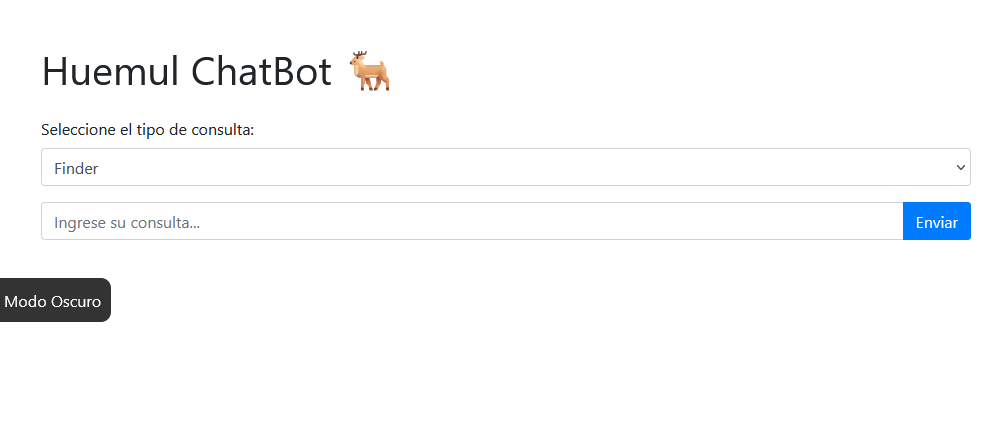
\includegraphics[width=.8\textwidth]{figures/website.png}
    \caption[]{\\
    {\scriptsize (Fuente: Elavoración propia)}}
    \label{fig:chatbot1}
\end{figure}

El prompt se procesa mediante una función de Embedding, empleando para ello OpenAI, siendo esta  
la función 'text-embedding-ada-002'. Esta función puede manejar hasta un máximo de 8191 tokens y 
produce un vector de 1536 dimensiones en forma de lista \cite{openai1}. Para determinar la similitud entre el 
vector del prompt y los vectores correspondientes a los documentos almacenados, se utiliza la función 
de similitud coseno presente en la \autoref{eq:similitudcoseno}.Esta mide el coseno del ángulo entre dos vectores,
Siendo estos $A$ y $B$ respectivamente, y este proporciona un valor que refleja su proximidad semántica entre el vector
del prompt y los vectores de todos los documentos almacenados en la base de datos ChromaDB.

\begin{equation}
    \text{similitud\_coseno}(\mathbf{A}, \mathbf{B}) = \frac{\mathbf{A} \cdot \mathbf{B}}{\|\mathbf{A}\| \|\mathbf{B}\|}
    \label{eq:similitudcoseno}
\end{equation}


\begin{figure}[ht!]
    \centering
    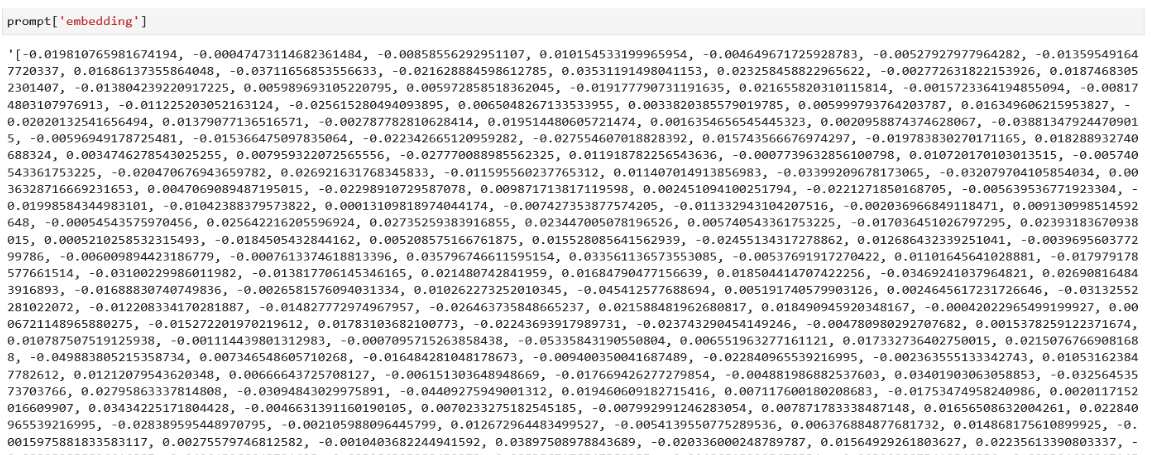
\includegraphics[width=0.9\textwidth]{figures/embedding1.png}
    \caption[Representación de un prompt luego de pasar por la funcion de embedding 'text-embedding-ada-002']{Representación de un prompt luego de pasar por la funcion de embedding 'text-embedding-ada-002'\\
    {\scriptsize (Fuente: Elavoración propia)}}
    \label{fig:chatbot1}
\end{figure}



\begin{figure}[ht!]
    \centering
    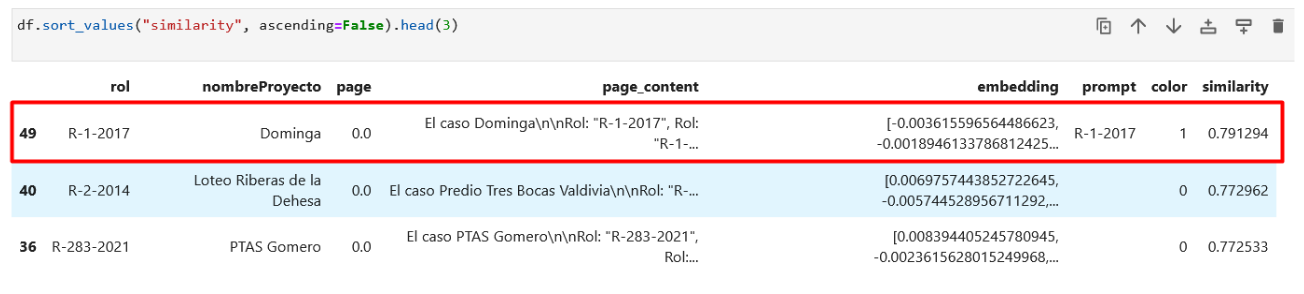
\includegraphics[width=0.9\textwidth]{figures/embedding2.png}
    \caption[]{\\
    {\scriptsize (Fuente: Elavoración propia)}}
    \label{fig:chatbot1}
\end{figure}



\begin{figure}[ht!]
    \centering
    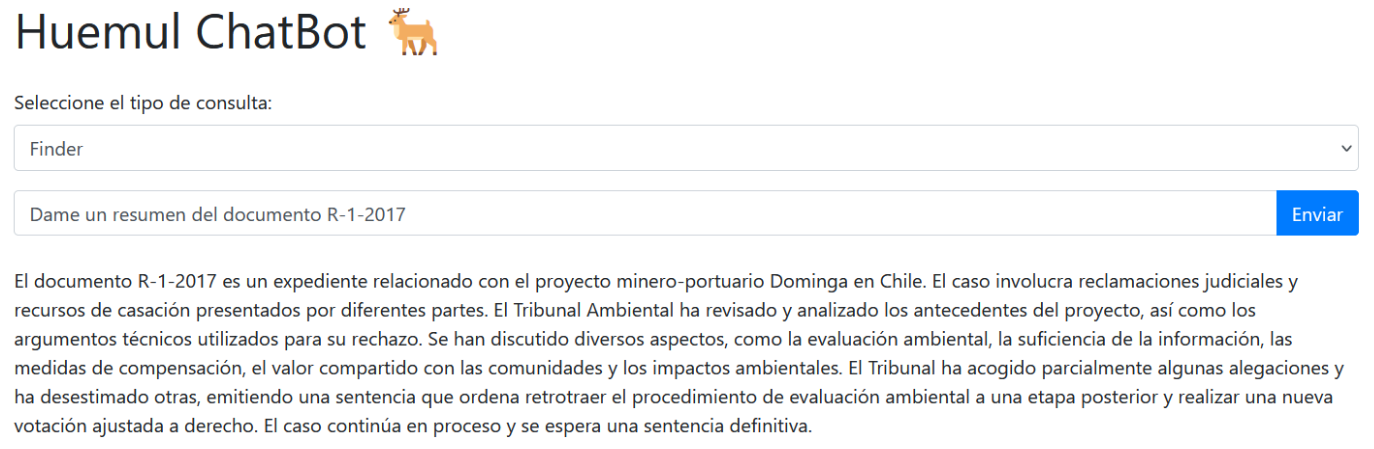
\includegraphics[width=0.9\textwidth]{figures/website2.png}
    \caption[]{\\
    {\scriptsize (Fuente: Elavoración propia)}}
    \label{fig:chatbot1}
\end{figure}